91. \begin{figure}[ht!]
\center{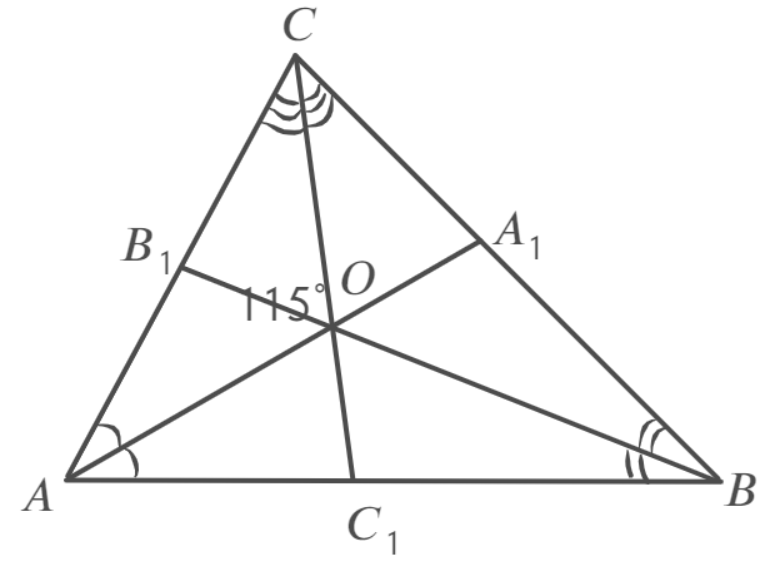
\includegraphics[scale=0.35]{g91.png}}
\end{figure}\\
Обозначим $\frac{1}{2}\angle B=y,\ \frac{1}{2}\angle C=z.$ Тогда из треугольника $AOC$ имеем $70^\circ:2+z+115^\circ=180^\circ,\ z=30^\circ.$ Значит, $\angle C=2z=60^\circ, \angle B=180^\circ-70^\circ-60^\circ=50^\circ, \angle AOB=180^\circ-70^\circ:2-50^\circ:2=120^\circ,\ \angle BOC=180^\circ-60^\circ:2-50^\circ:2=125^\circ.$\\
